\scalebox{.6}{
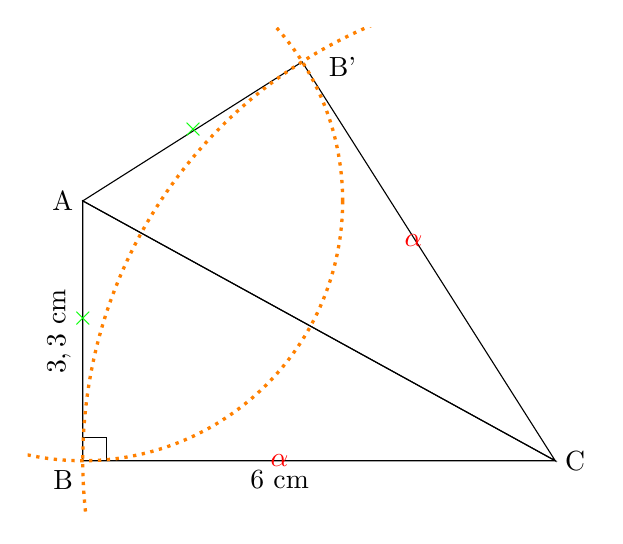
\begin{tikzpicture}	
  
    
\def \CharSize {1};
\def \BulletSize {1};

%on limite l'affichage de la figure
\clip (-0.7,5.5) rectangle (6.5,-0.7);

%triangles de base
\draw (0,0)--(6,0)--(0,3.3)--cycle;
\draw (6,0)--++(122.4:6)--(0,3.3)--cycle;

%angle droit
\draw (0,0) rectangle (0.3,0.3);

%longueurs et marquages égalité segments
\draw (2.5,0) node[below]{$6$ cm};
\draw (-0.3,2.3) node[left,rotate=90]{$3,3$ cm};
\draw (4.2,2.8) node[color=red]{$\alpha$};
\draw (2.5,0) node[color=red]{$\alpha$};
\draw (0,1.8) node[color=green]{$\times$};
\draw (1.4,4.2) node[color=green]{$\times$};

%arcs de cercle : on fait des cercles et on \clip l'image!!
\draw [dotted, very thick, color=orange](6,0) circle (6);
\draw [dotted, very thick, color=orange](0,3.3) circle (3.3);

%les points
\draw (0,0)[below left] node{B};
\draw (0,3.3)[left] node{A};
\draw (6,0)[right] node{C};
\draw (3,5)[right] node{B'};


\end{tikzpicture} 
 } %fin de la scalebox